% \documentclass[conference]{IEEEtran}
\documentclass[17pt]{article}
\usepackage[english]{babel}
\usepackage[utf8]{inputenc}
\usepackage{hyperref}
\usepackage{cleveref}
\usepackage{graphicx}
\usepackage{pgfplots}
\usepackage{biblatex}
\usepackage{fancyhdr}
\usepackage{listings}
% STYLE IEEE TO USE
\addbibresource{./References/referinte.bib}
\graphicspath{ {./images/} }

\newcommand{\coo}{\ensuremath{\mathrm{CO_2}}}

\begin{document}

\thispagestyle{empty}
\begin{center}
\begin{figure}[h!]
\vspace{-20pt}
\begin{center}

\includegraphics[width=100pt]{FMI-03.png}
\end{center}
\end{figure}

\lstdefinelanguage{json}{
  basicstyle=\ttfamily\footnotesize,
  numbers=left,
  numberstyle=\scriptsize,
  stepnumber=1,
  numbersep=8pt,
  showstringspaces=false,
  breaklines=true,
  frame=lines,
  backgroundcolor=\color{white},
  morestring=[b]{"},
  stringstyle=\color{blue},
  commentstyle=\color{red},
  keywordstyle=\color{black},
  morekeywords={null,true,false}
}

{\large{\bf WEST UNIVERSITY OF TIMI\c SOARA

FACULTY OF MATHEMATICS AND COMPUTER SCIENCE

BACHELOR STUDY PROGRAM: Computer Science}}

\vspace{120pt}
{\huge {\bf BACHELOR THESIS}}

\vspace{160pt}
\end{center}

{\large\noindent{\bf SUPERVISOR: Todor Ivașcu
\hspace{30pt} GRADUATE: Mihai \indent \indent \indent \indent
\indent \indent \indent \indent \indent \indent \indent \indent 
\indent \indent \indent Andrei Gherghinescu}

\noindent Prof./Conf./Lect. Dr. Firstname Lastname \hfill 
\noindent  Firstname Lastname
}

\vfill
\begin{center}
{\bf TIMI\c SOARA

2023}
\end{center}
\newpage
\thispagestyle{empty}
\begin{center}
{\large{\bf WEST UNIVERSITY OF TIMI\c SOARA
		
FACULTY OF MATHEMATICS AND COMPUTER SCIENCE
		
BACHELOR STUDY PROGRAM:  Computer Science}}

\vspace{200pt}
{\huge {\bf Traffic Manager }}

\vspace{153pt}
\end{center}

{\large\noindent{\bf SUPERVISOR: Todor Ivașcu
\hspace{30pt} GRADUATE: Mihai \indent \indent \indent \indent
\indent \indent \indent \indent \indent \indent \indent \indent 
\indent \indent \indent Andrei Gherghinescu}

\noindent Prof./Conf./Lect. Dr. Firstname  Lastname\hfill
\noindent Firstname  Lastname}


\vfill
\begin{center}
{\bf TIMI\c SOARA

2023}
\end{center}

\newpage
\normalsize{}

\section*{Abstract}
\indent \indent
The paper introduces an intelligent system for traffic
signal applications that is designed to be as adaptive
as possible and combines multiple technologies.
At base, it is programmed on an micro controller and it
uses fuzzy logic, but can be upgraded. This can be done by
linking other hardware components to it with the help of a
configuration file. So we can utilize multiple technologies
like image recognition or speed/radio detection and get the
best from all of them.\\
\indent The system aims to be used in real time
traffic scenarios, as an affordable and upgradable option,
to decrease the waiting time at crossroads.
This would lead to shorter travel times from point
A to point B and would have a significant impact not only
on our daily lifes, but on the environment as well.

%add more to abstract sadly
\pagebreak

\tableofcontents

\pagebreak

\listoftables

\pagebreak

\listoffigures
\pagebreak

\section{Introduction}
\indent \indent
Intersections are the points where two or more
routes overlap with one another. As a result, for drivers, 
they act as an obstruction for smooth traffic
flow especially within urban areas where the
infrastructure demands them the most. This leads to
traffic interruption, congestion, and poor control and
management of the traffic.\\
\indent \indent
To minimize the amount of time lost at crossroads while
maintining the safety of the drivers, Intelligent
Transportation Systems (ITS) were developed.
One major impact that can be seen as a result is the
reduction of \coo\ car emissions. You may think that
this wouldn't be relevant when the era of combustion
engines comes to an end, but there are so many other
bennefits apart from this. For example, the less time
it takes for resources to travel from a provider to a
manufacturer, the faster the production can start so
it also has a huge impact on the global economy.\\
\indent \indent
As it's occurrence is noticed the most in urban areas,
the problem is currently being tackled in concordance 
with the smart city concept. A smart city is defined as an
ultra-modern urban area that aims to improve the overall life
quality of citizens. It is based on different arhitectural
approaches that involve modernizing and upgrading our current 
environment by applying new concepts and technologies on top
of the ones currently in use.\\

\section{Overview of the Technology Developed}

\indent \indent
To better understand the problem we must first know what solutions
were used to fix the issue through out the time and how they evolved.\\
\indent \indent
The first solution that was put in use was created long time ago and required
the use of actual human resources to control the traffic. Policemans were
responsible to manage the traffic at junctions. Once with the  technological
era, we were able to remove the need of this kind of resources by creating
autonomous systems that alternate between STOP and GO phases. The design of the 
systems was pretty simple and straightforward, we would use lights to signal 
those phases. Red lights were matched with the STOP phase, green ones with the
GO phase. To prevent collisions and maintain drivers safety amber was
introduced as well. It notifys the drivers that STOP and GO phases will soon
switch and they should take the corresponding measures.\\
\indent \indent
As the time passed by and the number of cars on the road increased drivers 
started experiencing traffic jams scenarios. Also there was clearly a better
option then having a standard fixed time to change the lights. Many times
the green signal was turned on even though there were no cars crossing that
given road while on the other crossing roads there were actual drivers waiting.
Something had to be done, a more efficient way had to be found, but at what
cost? If we wanted to develop better solution we would need the help of
expensive hardware components.\\
\indent \indent
We reach the point in time when a new discovery was made: bugdet units based
on  microcontrollers, sensors and recievers \cite{Deshmukh2016} that were
cable of running advanced algorithms (Figure ~\ref{fig:PI}). So all that was left was to develop 
new solution and use them to design an intelligent Traffic Light Control
System (TSC)\\
\begin{figure}[h!]
    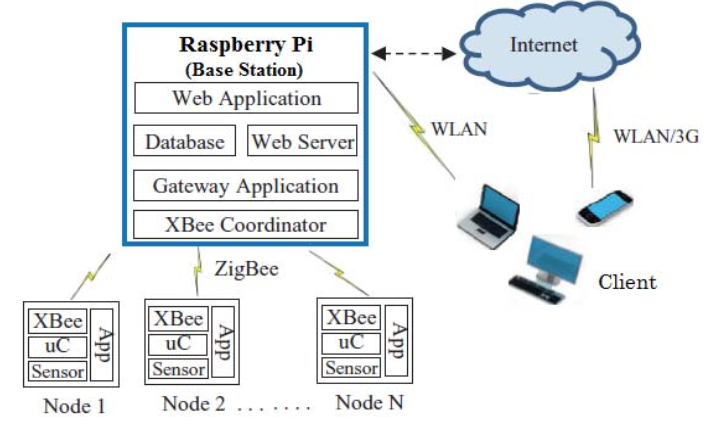
\includegraphics[width=\textwidth]{PiSystems.png}
    \caption{Rasberry PI based system \textcopyright }
    \label{fig:PI}
\end{figure}
\\

\indent \indent
By the time writing, TSC is an active research topic that proved to be really
challenging. Continuous work has been done on designing and developing
intelligent traffic signal control systems that could address the issue.\\
\indent \indent
So new methods and advanced systems based on fuzzy logic, evolutionary
algorithms, image processing, neural network and many other algorithms have
been proposed by the researchers to solve this TSC problem \cite{Tomar2022}.
All of the methods aimed to reduce the overall waiting time and prevent traffic
jams from occurring while maintaining drivers safety. In this section we will
discuss about some of the methods that were put in to use and their ups and
downs. After describing each and every tehnology we will have a brief
comparison to highlight some of their characteristics.

% sectiunile devin capitole
\pagebreak
\subsection{Object recognition based systems}
\indent \indent
One way to determine traffic scenarios was done with
the help of cameras. To be more specific we wanted to 
calculate the traffic waiting queue by using the 
images provided by the cameras. This problem was addressed by the
help of vehicle tracking and image segmentation algorithms.
\begin{figure}[h!]
    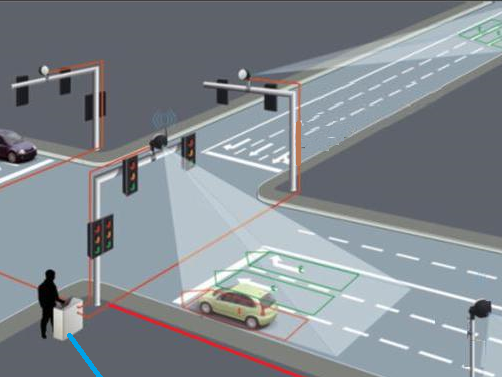
\includegraphics[width=\textwidth]{ObjectRecognitionSystemRepresentation.png}
    \caption{Object Recognition Based Traffic System Model \textcopyright}
    \label{fig:ObjectRecognitionSystem}
\end{figure}
\\
\indent \indent
However, the techniques used to solve the problem
become ineffective for real-time operations because of the 
computational complexity and longer execution time. Also,
some are not even able to operate in bad weather conditions,
so they were doomed to failure. Studies had shown that whenever
visibility is reduced due to rain, fog or other external factors that
the pecentage of vehicles that will be detected will significantly drop.
\cite{Sheeny2021} \\
\indent \indent
Even if the problems stated above were known,
neural networks systems have been developed with the help of
object recognition algorithms.
They were designed to predict the upcoming traffic volume
from a X-min daylight traffic flow on an expressway. 
Like so we would be able to overcome the high computational
complexity of the algorithm by avoiding 
recalculations. This lead to high memory needs,
that could not be overcomed, so this approach is
unsuitable for real-time systems.\\
\indent \indent
To sum it up, unless the memory
issue is somehow fixed in the near future they are not a
viable option for tracking vehicles.\\

\subsection{Vehicle sensor detection based systems}
\indent \indent
Another approach would be to collect data about the vehicles 
approaching junctions with the help of GPS sensors.
(Figure ~\ref{fig:SensorRecognitionSystem})\\
\indent \indent
One way to do it is to track the position, speed and direction of the given
vehicles. Sadly, this method would work only for a road network,
it can not solely control the traffic signal timing for just one junction. 
This is due to the high speeds that vehicles travel at and the time 
complexity of the  main algorithm.\\ 
\indent \indent
Another way to do it is to monitor the arrival and departure of vehicles at a
junction. This can be done with the help of sensors and traffic servers.
Like so we could use embedded technology to record the GPS data and send it to
the traffic monitoring system through GSM/GPRS. The drawbacks of this method
are the fact thats it involves very high implementation cost and, sadly, some
vehicles can not be tracked using radio detection systems. This problem can
be also aproached with the help of in-road sensors, but it would require even higher 
costs as you would need often change the sensors because roads often need to be
rebuilt due to wear or ongoing costructions.

\begin{figure}[h!]
    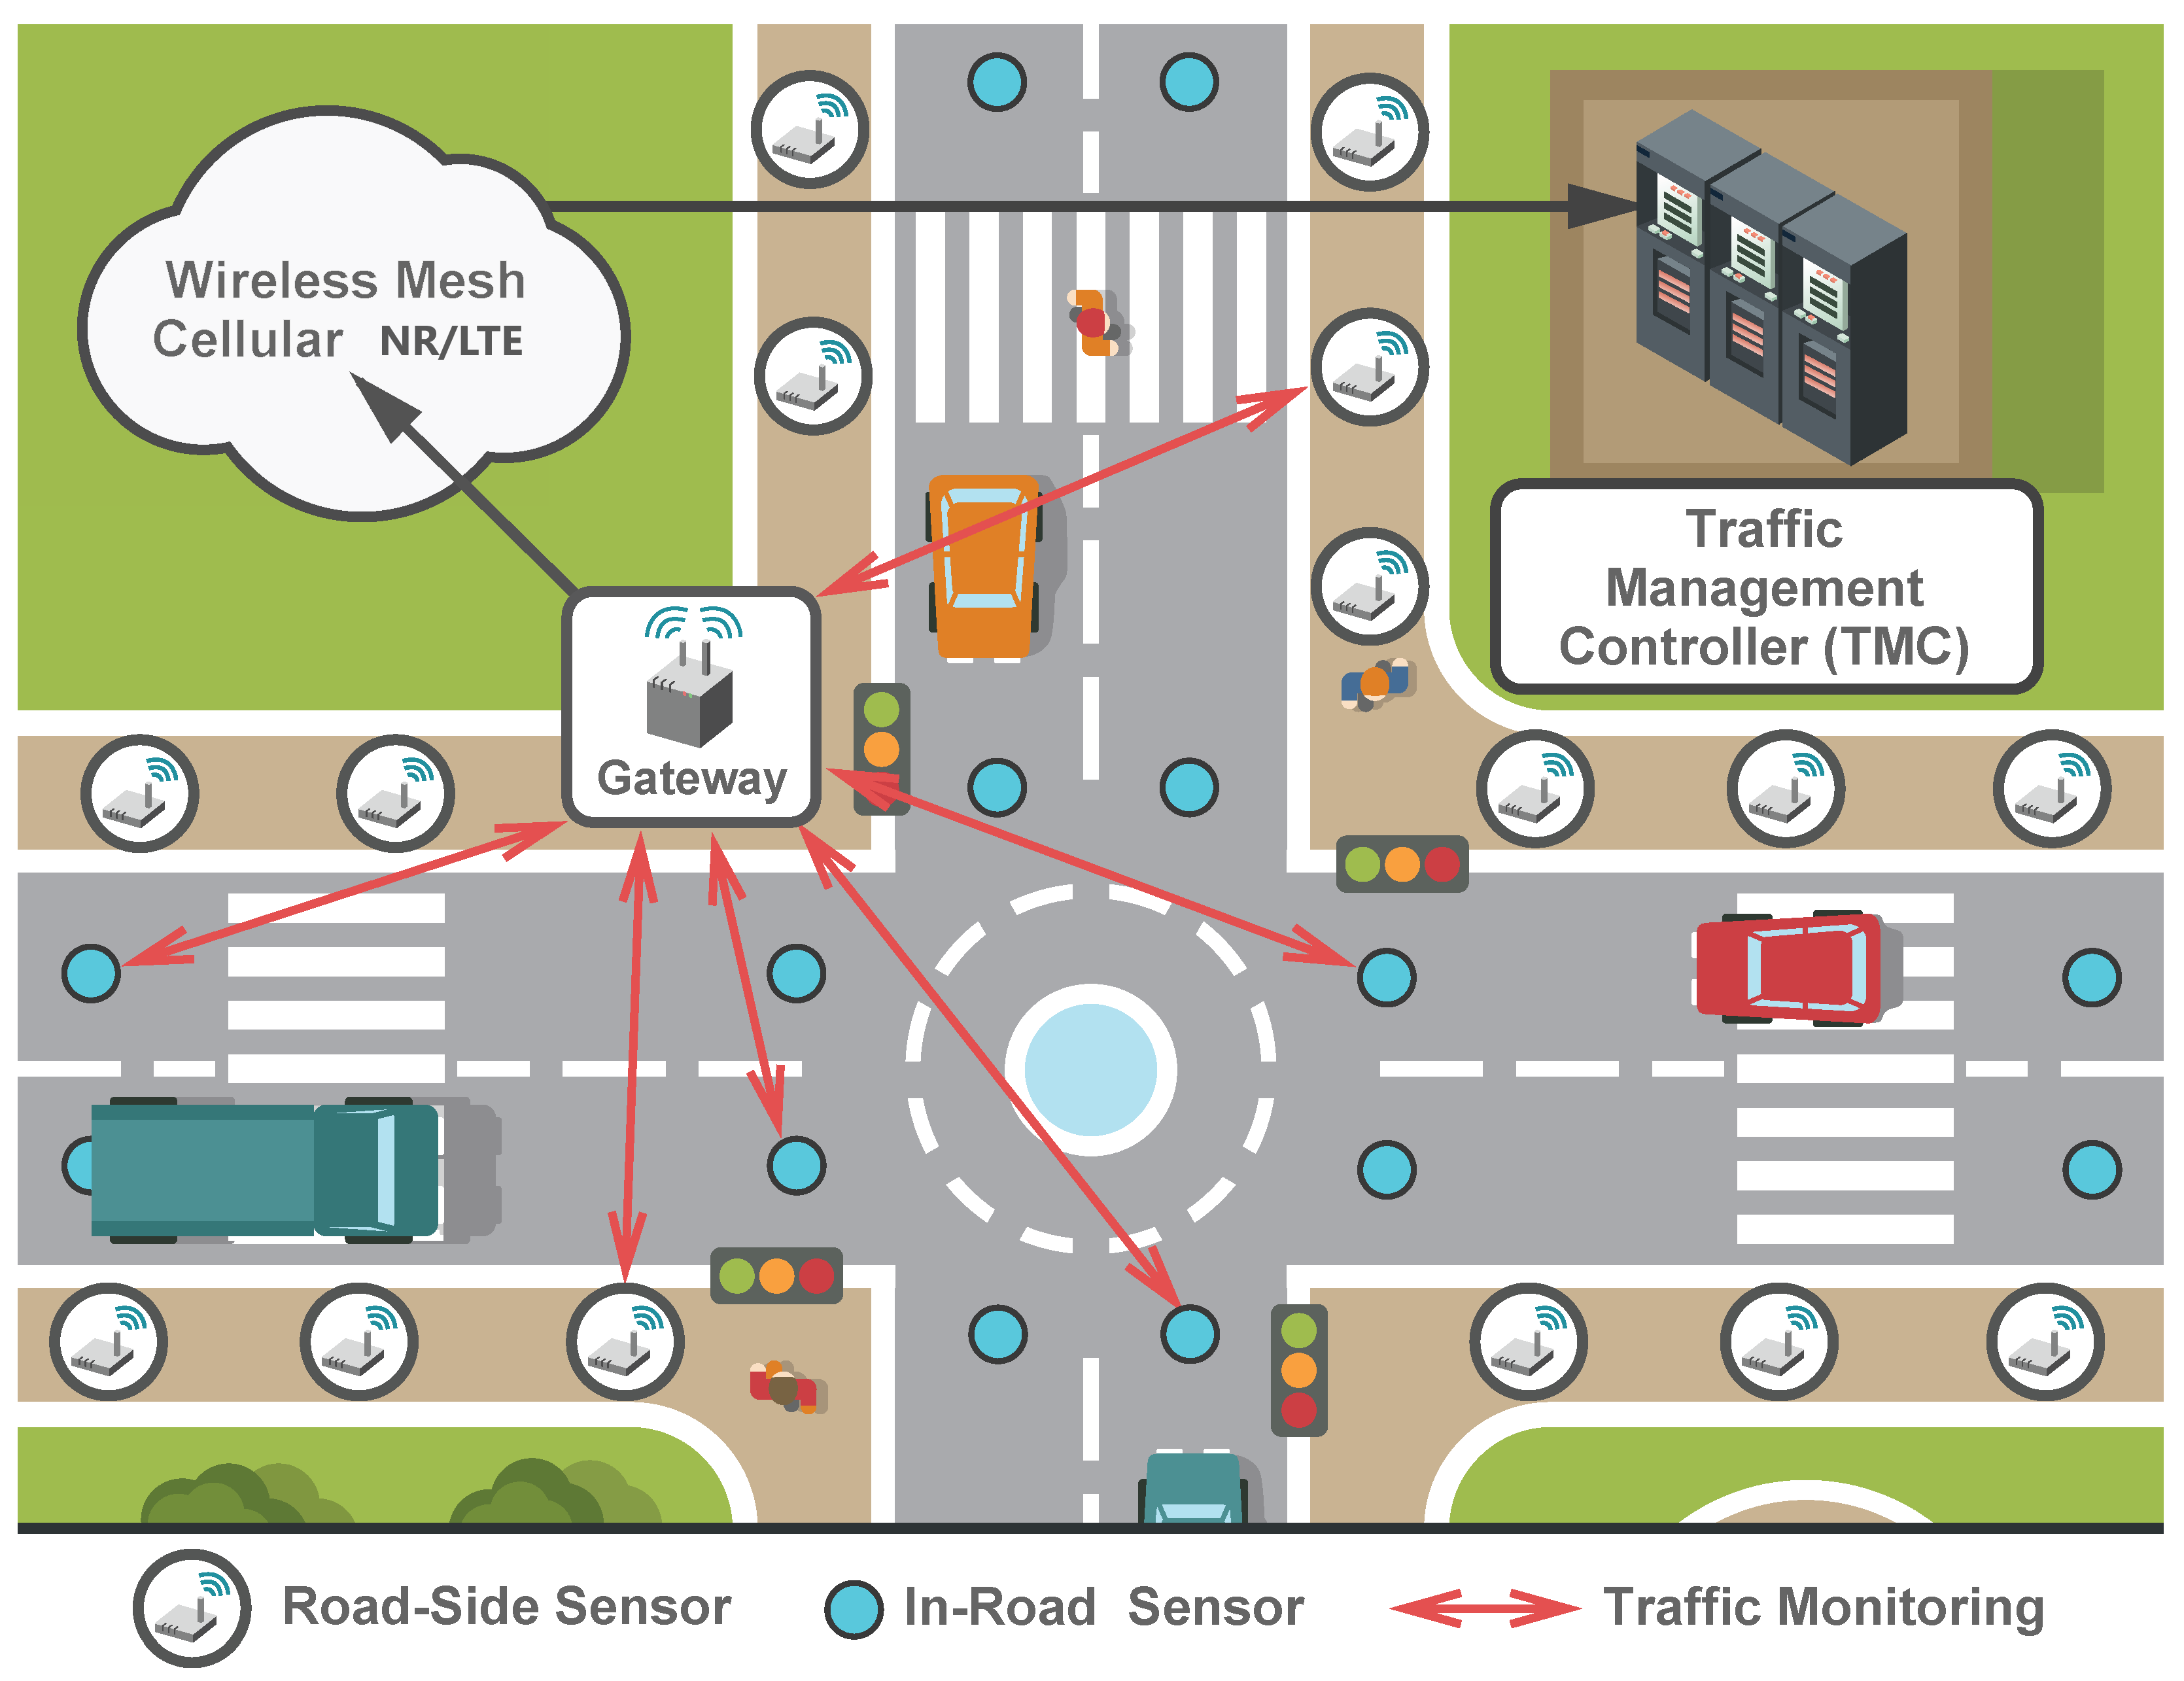
\includegraphics[width=\textwidth]{SensorsBasedTrafficControlSystemRepresentation.png}
    \caption{Sensor Based Traffic System Model \textcopyright}
    \label{fig:SensorRecognitionSystem}
\end{figure}

\pagebreak

\subsection{Traffic Lights Synchronization based systems}
\indent \indent
Traffic Lights Synchronization (TSC) \cite{Tomar2022} systems aim  to minimize
the number of STOP and GO occurrences by adapting the traffic light phases at junctions.
It is a technique in which a vehicle traveling along one side of the road at a specific
speed can continue to the opposite end of the road indefinitely by obtaining the maximum
number of green lights at the intersections. Studies had shown that in comparison with
other fixed time and non-synchronized traffic control strategies it reduces overall travel
time by up to 39\%. \cite{ALEKO2019}\\
\indent \indent
Just like most of the others methods, it collects and procces data from real traffic
scenarios to determine the green light timer. When vehicles pass through a juction the
green light timer for the following juctions decreases by a certain amount
(Figure ~\ref{fig:TrafficSignalSynchronization}). As with the other roads present at
the juction, the red light time increase to guarante the continuous motion of already
travelling cars. This can be done for mutiple levels of traffic depending on how many
junctions do you want to synchronize with one another, but must of the the times it
was handled as a 2 level system.
\begin{figure}[h!]
    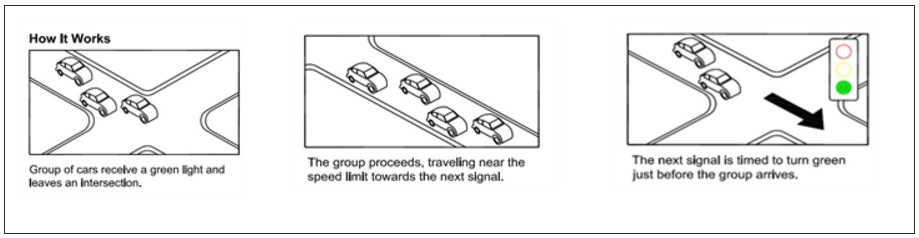
\includegraphics[width=\textwidth]{TrafficSignalSynchronization.jpg}
    \caption{Traffic Signal Synchronization Model \textcopyright}
    \label{fig:TrafficSignalSynchronization}
\end{figure}\\
\indent \indent
Multiple approaches to implement this kind of systems were made with the use of
varios AI algorithms and already known data collecting methods but the result are
mostly the same. This method would lead to longer red signal time, but will reduce
the overall waiting time when travelling long distances. One other advance to keep in
mind is that, as result of this phenomenon, the wear of the vehicles will be
drastically reduced.\\
\indent \indent
The main disadvantages of this method is the fact that you will eventually have to
prioritize one route. This would be problematic if multiple main rouds colide with
one another. Also, the algorithm will not always provide an optimal solution as
drives following sideroads may have longer waiting times. One more thing to keep in mind
is that this method is reliant on drivers speed consistency. Most of the cases, there 
will be a decent amount of speeding vehicles that will not be able to pass multile
junctions without any kind of stops as algorithm does not expect this from drivers side.

\pagebreak

\subsection{Fuzzy Intelligent Traffic Signal Control System}
\indent \indent
Fuzzy Intelligent Traffic Signal Control (FITS) \cite{Teo2010} \cite{Jin2017}
systems were originally designed to mimic a human policeman in controlling
traffic lights at an intersection. They are systems that take
different types of traffic input and apply fuzzy rules to 
manage the traffic. Like so data is converted into fuzzy truth
values between 0 and 1. For instance, the green light extension
time can be modeled by a number of fuzzy sets including “none”,
“short”, “moderate” and “long”. The only thing that you are left to do is
to define your membership functions for the given set. For example we can
use the following functions to do so:\\

\begin{equation}
    "none" - f(q) = max(min((10 - q) / 10, 2), 0)
\end{equation}

\begin{equation}
    "short" - f(q) = max(min(q / 10, (20 - q) / 10), 0)
\end{equation}

\begin{equation}
    "medium" - f(q) = max(min(q / 5, (30 - q) / 5), 0)
\end{equation}

\begin{equation}
    "long" - f(q) = max(min((50 - q) / 10, q / 2), 0)
\end{equation}


Like so we would alternate base on other fuzzy values or randomly, between
choosing "none", "short", "moderate" and "long" fuzzy values, to determine 
the time that out green light should last using.\\
\indent \indent
Depending on the actual improvements of the traffic flow the algorithm will 
adapt, altering it's member functions and decreasing/increasing the odds to 
chose one specific fuzzy value from the set. One big advantage that this would 
lead to is that FITS mitigates the negative effects of detection malfunction
by predicting the traffic states at the whole intersection by simulating real
time traffic scenarios. So FITS may be able to run withot any kind of additional
hardware, leading to huge cost advantages.\\
\indent \indent
Despite all of the bennefits presented above, as with any AI based algorithm,
it takes a lot of time for the algorithm to improve itself and the upgrade.
Also the chance to upgrade is very reliant on traffic conditions. Furthermore, 
even if the algorithm has been running for a long time, it still can choose a
non optimal solution that may or may not lead to traffic jams. 

\pagebreak

\subsection{Dedicated Short-Range Communications systems}
\indent \indent
To explain why this kind of systems would work, first we have to understand what
are Dedicated Short-Range Communications (DSRC) \cite{Zhang2018}
\cite{Tomar2022}. DSRC are one-way or two-way wireless communication channels
specially designed for use in automobiles that are mostly used by ITS to
comunicate with other vehicles or infrastructure technology. They operate on
the 5.9 GHz band of the radio frequency spectrum and are effective over short
to medium distances.\\
\indent \indent
One technique that was developed with the help of DSRC is the Virtual Traffic
Light (VTL) approach. VTL is a biologically-inspired approach to traffic
control that relies on Vehicle-to-Vehicle (V2V) communication by using the
Signal Phase and Timing (SPaT) message and Basic Safety Message (BSM) from
the DSRC OBU. (Figure ~\ref{fig:DSRCRadio})
\begin{figure}[h!]
    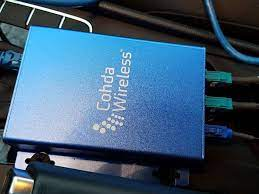
\includegraphics[width=\textwidth]{DSRCRadio.jpeg}
    \caption{Dedicated Short-Range Communications Radio \textcopyright}
    \label{fig:DSRCRadio}
\end{figure}\\

\indent \indent 
The radio is capable of broadcasting several messages defined by the SAE 2735
\cite{Kenney2011IOT} protocol with the most important beeing BSMs. This kind of 
messages contain vehicle's current information (GPS location, speed and where they
are heading) that are associated with a temporary ID. As a result, by broadcasting
BSM messages we are able to detect the vehicles approaching the intersection in a
continuous manner, unlike traditional methods that only detect the presence of the
vechile using loop detectors.\\
\indent \indent 
You can image the cars beeing "moving routers", and the junctions beeing
"stationary routers". Whenever one "gateway" or in our case one traffic route is
overfilled with vehicles it blocks the others and starts letting them pass just like
RIP protocol. Like so we are not actually introducing new sorts of technology that may
or not fail, we just adapt already existing algorithms that proved to be great
solutions to fit one specific use case.
%NOT SURE IF RIP IS THE RIGHT ONE DOUBLE CHECK LATTER!!
\begin{figure}[h!]
    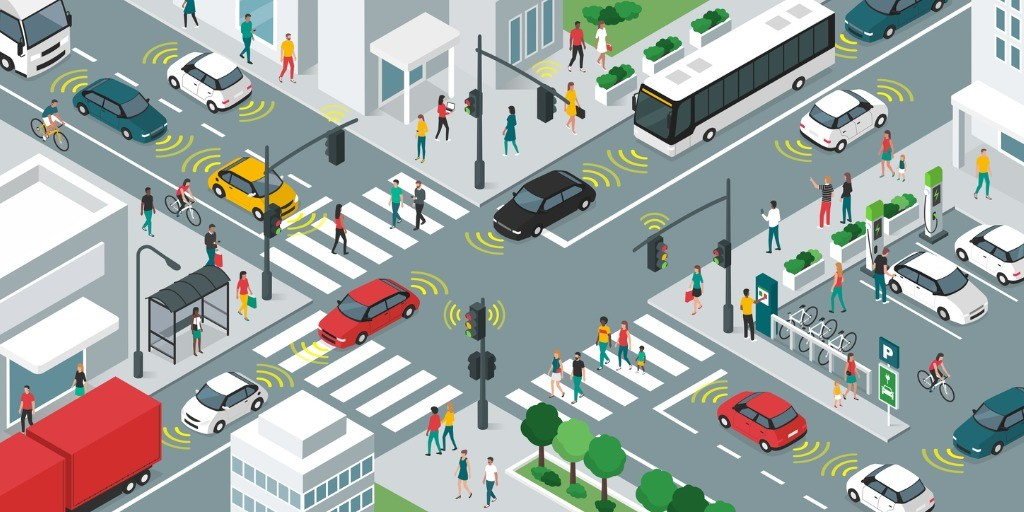
\includegraphics[width=\textwidth]{DSRCSystemModel.jpg}
    \caption{DSRC Based System Model \textcopyright}
    \label{fig:DSRCSystemModel}
\end{figure}\\

\indent \indent
With the help of this approach we can drastically reduce
the implementation costs as it does not require any kind of additional
expensive hardware components. Furthermore, it is robust against weather conditions
and easy to mantain. Extensive simulations have shown that this kind
of technology can reduce daily commute time in urban areas by more than 30\%.
Different aspects of VTL technology, including system simulation, carbon
emission, algorithm design and deployment policy have been researched in the
last few years. \cite{Neudecker2012}\\
\indent \indent
The drawback of this approach is that it requires vehicles
to support DSRC technologies, which is not possible at the present time.
Furthermore, V2V communications in VTL could come across partial obstruction by
a physical object present in the innermost Fresnel zone (non-LoS conditions),
which makes rapid decision making extremely challenging. However, even if DSRC
technology isn't totally supported by vehicles and we might colide with non-Los
conditions, it proved to be effective in reducing the average waiting time at
juctions. So, maybe the next step on improving traffic flow, would be to create
an infrastructure for this kind of technologie, but only time will tell. In the mean
time the best thing we can do is to develop a cost-effective transition scheme
between current traffic control systems and VTL systems.

\pagebreak


% tables for all comparatie

% \paragraph{Advantages}
% \paragraph{Disadvantages}

\section{A new flexible economic approach}
\indent \indent
We belive that the future of traffic light management will be
based on DSRC like signals. No matter if it will still be based 
on DSRC, 5G or even 6G will take lead, we aim to provide a some kind of
software system that would be able to handle any kind message based 
tehnology. Also, because at the given moment, the infrastructure for
DSRC systems hasn't been fully developed and deployed we want to
provide a economic approach to the given problem that would also bennefit
on the already working systems, but also can simulate the already
working traffic light management protocol.\\
\indent \indent
Even if DSRC will be fully deployed on a globas bases, there will still be
alot of poor countries that will have a hard time upgrading their infrastructure.
Because of that, we wanted to be able to have a working system even without 
investing any kind of money. Thing about a PC for example. Even one of the worst
ones can run an OS and if you want to updgrade them, to make it run faster or
handle a newer software, you would just add or replace a component with a better
performing one. Not only you will be able to add "performance boosts" as needed
to your given infrastructure but think about the scenarios when something goes bad?
What if one of your component goes down and for example the traffic light will
be stuck on red until someone comes and fixes it. That would lead to a
HUGE traffic jam.\\
\indent \indent
We also want to be able to take advantage of already working DSRC compatible
vechiles without adding any kind of new hardware  and be able to 
disable the additional protocols and move to a fully DRSC based
system if needed.

Sounds great, right? This is how we designed it. The system will have \textbf{4 major
components}: \textbf{2 types of clients}: one stationary one and one moving one, 
"attached" to our vechiles; \textbf{2 types of servers}: one that would manage the
position of the clients and redirect them to the corresponding servers
and one that would handle all of the messages and change the actual traffic lights.
For the simplicity on things we will name them as follows:
\begin{itemize}
    \item \textbf{Traffic Observer (TO)} - the stationary client.
    \item \textbf{Vehicle Tracker (VT)} - the moving client
    \item \textbf{Junction Main Server (JMS)} - the server that handles the traffic lights
    \item \textbf{Proxy} - the server that will guide the clients to the corresponding
    servers
\end{itemize}

\pagebreak
The system would work as follows: We would constanly have a TCP-IP connection
between our clients and the corresponding JMS. Once they are connected
clients would send various data about the traffic that would be further 
proccesed by the JMS and traffic lights would be changed accordingly. The
TO would be responsible for sending data about the traffic on it's road and the 
VT would be responsible for sending it's own data to the server (Figure ~\ref{fig:UC_DiagramAll}). 
We also handled the cases when there is an emergency ongoing like any kind of
special vehicles crossing the junction but we will talk later about this
because it requires some more attention as it can be easily exploited if not 
handled right. Just imagine any kind of cars beeing treated like an ambulance
on duty, you would just be able to pass freely any kind of junction without 
ever waiting at the red light.\\

\begin{figure}[h!]
    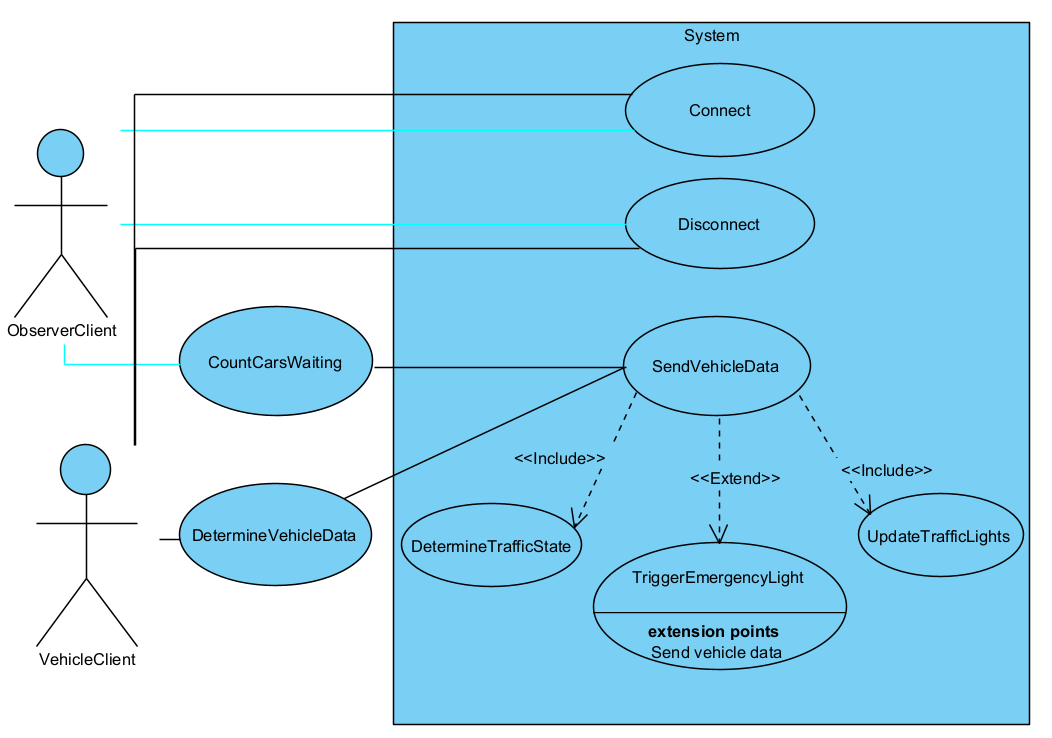
\includegraphics[width=\textwidth]{UC/UCDiagram.png}
    \caption{All UC Diagram}
    \label{fig:UC_DiagramAll}
\end{figure}

\pagebreak

\subsection{Proxy}
\indent \indent
The first problem that needs to be addressed is the fact that VTs will 
constanly have to switch between JMSs, but how do we know what server to 
connect to? We do not want to connect to each and every server in the 
covered area and start broadcasting mostly useless message. The answear
would be that each client will know the main server off the system, that
would act just like a proxy and redirect them to the corresponding JMS.
For that we would need to store the JMS coordinates in one or multile
database. The VT would need to just send its own coordinates and the
direction they are heading, as a result the proxy would provide de IP
address of the corresponding JMS (Figure ~\ref{fig:UC_Connect}).\\
\indent \indent
As we want this to be scaled on a global level, the system supports
horizontal scalling, as we can just stack proxys one on top of the 
other and instead of having stored only to the JMS coordinates we 
will also store all the proxys that are in the subarea of the owner. To 
not overload any kind of servers we also implemented a load balancing
mechanism that prevents this kind of issue.
\begin{figure}[h!]
    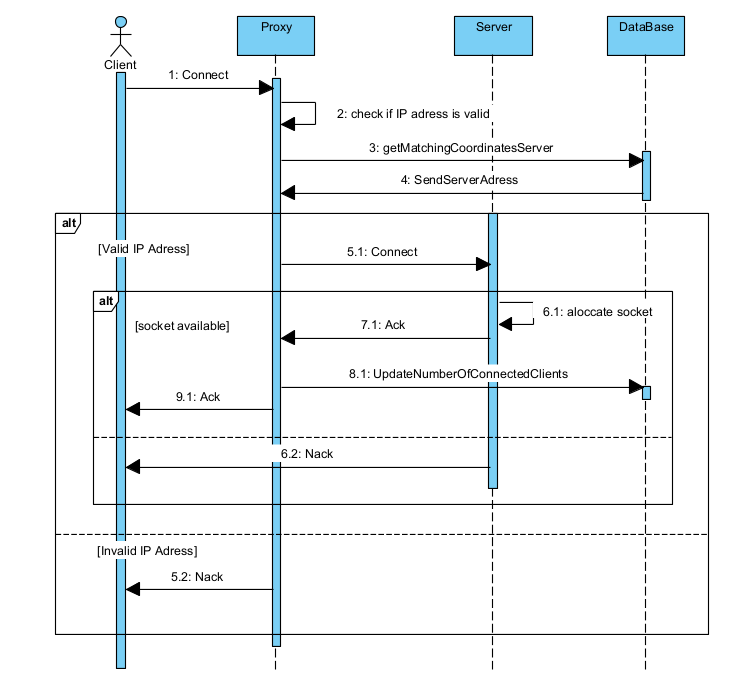
\includegraphics[width=\textwidth]{UC/Connect.png}
    \caption{UC: Connect}
    \label{fig:UC_Connect}
\end{figure}

\pagebreak

One thing this can lead to is a 
better surveillance of the vechiles that aren't suppose to be on the 
road in the first place. The IP address of a given vechile can be "banned"
and if it tries to connect to the JMS the message will be ignored
and not only the JMS will not count the waiting vechile, sometimes 
leading to longer waiting times for the individual that is driving the
vechile and broke the law, but also like this we would have the proof
that he broke the law so we would be able to further punish him. We can lower the number of cars driving on the public
roads that do not respect safety norms and reduce the number of
accidents. For this to work we will need to also disallow owners to 
change their hardware without any kind of approval as a new radio
would lead to a different IP address and this would be problematic.\\
\indent \indent 
Once passing the area of coverage of that given junction we would also need
to disconnect from that given JMS (Figure ~\ref{fig:UC_Disconnect}).


\begin{figure}[h!]
    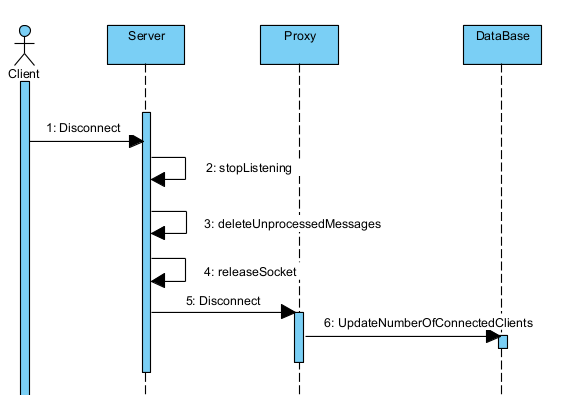
\includegraphics[width=\textwidth]{UC/Disconnect.png}
    \caption{UC: Disconnect}
    \label{fig:UC_Disconnect}
\end{figure}

\pagebreak

\subsection{Traffic Observer}
\indent \indent
The second thing we need to do is provide a way to detect the
waiting vechiles withot the help of DSRC messages. This can be
done in mutiple ways, but for the simplicity of things and to keep
costs as low as possible we went with an camera based system.
The way it works is as follows: a camera is mounted on the road we 
want to keep track of, that is connected to a microcontroller that can 
run our software.

\begin{figure}[h!]
    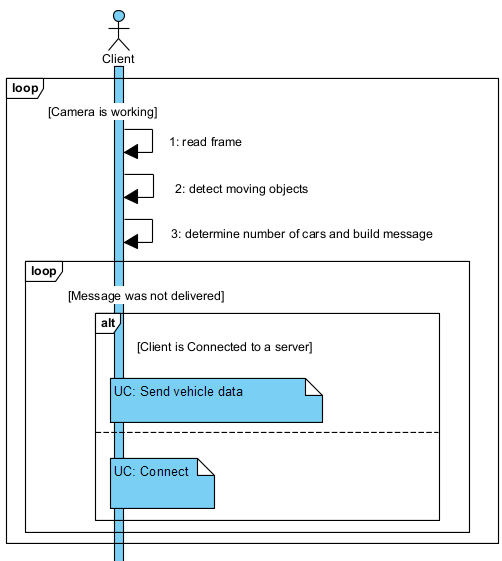
\includegraphics[width=\textwidth]{UC/ProcessImageAndFindTheCars.png}
    \caption{UC: Find cars from provided images}
    \label{fig:UC_FindCars}
\end{figure}

\pagebreak
With the help of the provided images we first and
foremost detect the moving objects on the given frames and second of all
determine if that moving object is or is not a vechile (Figure ~\ref{fig:UC_FindCars}).
Like this we can speed up the image detection process as we will have less pixels
to keep track off. The car detection speedup of the movement detection can be 
seen in Figure ~\ref{fig:Comparison}. The blue line represents the amount of cars 
detected with it running and the red one without it.
%TO PROVIDE REAL DATA WHEN APP IS DONE
\begin{figure}[h!]
    \centering
    \begin{tikzpicture}
        \begin{axis}[
            xlabel={$seconds$},
            ylabel={$cars-counted$},
        ]
            \addplot[color=red]table {testData/dataNoMovementRecognition.txt};
            \addplot[color=blue]table {testData/dataMovementRecognition.txt};
        \end{axis}
    \end{tikzpicture}
    \label{fig:Comparison}
\end{figure}

\subsection{Vehicle Tracker}
\indent \indent
We want to be able to handle DSRC signals. But how can we achieve that?
We do not want to add additional hardware requirments as this will just
make the deployment of our app much much slower and more costly. Well,
we make use of already integrated hardware components, to be more specific we 
make use of the radios and GPS trackers. With the use of the GPS we get the
coordinates of the vehicle as well as it's heading. The radio allows us to
establish TCP-IP connection and send messages. So the only things that is left to do
is to download our app and keep it running while travelling.\\
\indent \indent
To identify the vehicles we allocate them an IP adress when installing the app. But how can we
make sure the user isn't amble to freely change their adress? We would want an "immutable
storage space" to achieve that. To do so we require the manufacturer to encrypt their storage
data so that only they will be able to modify it if needed. We just talked about the fortunate
case, if for example we just unplug the radio module from the car how would we be able to send
data in the system? Well we couldn't, but thats not necessarily what we want to achive. We want
to prevent the sending of invalid data to the system and we achived that for now, when it comes
to actual vehicles. Other faulty scenarios like driving a car without a radio, basically in
"incognito mode", should be punished by the law and is something that we just shouldn't handle.

%PHOTO HERE
\pagebreak
\subsection{Junction Main Server}
\indent \indent
To handle all of those messages and change the actual flow of traffic we
need to have a main command unit that acts as a server. Now 
that we know about all the components of the system we can 
start vizualing it(Figure ~\ref{fig:System_sketch}).

\begin{figure}[h!]
    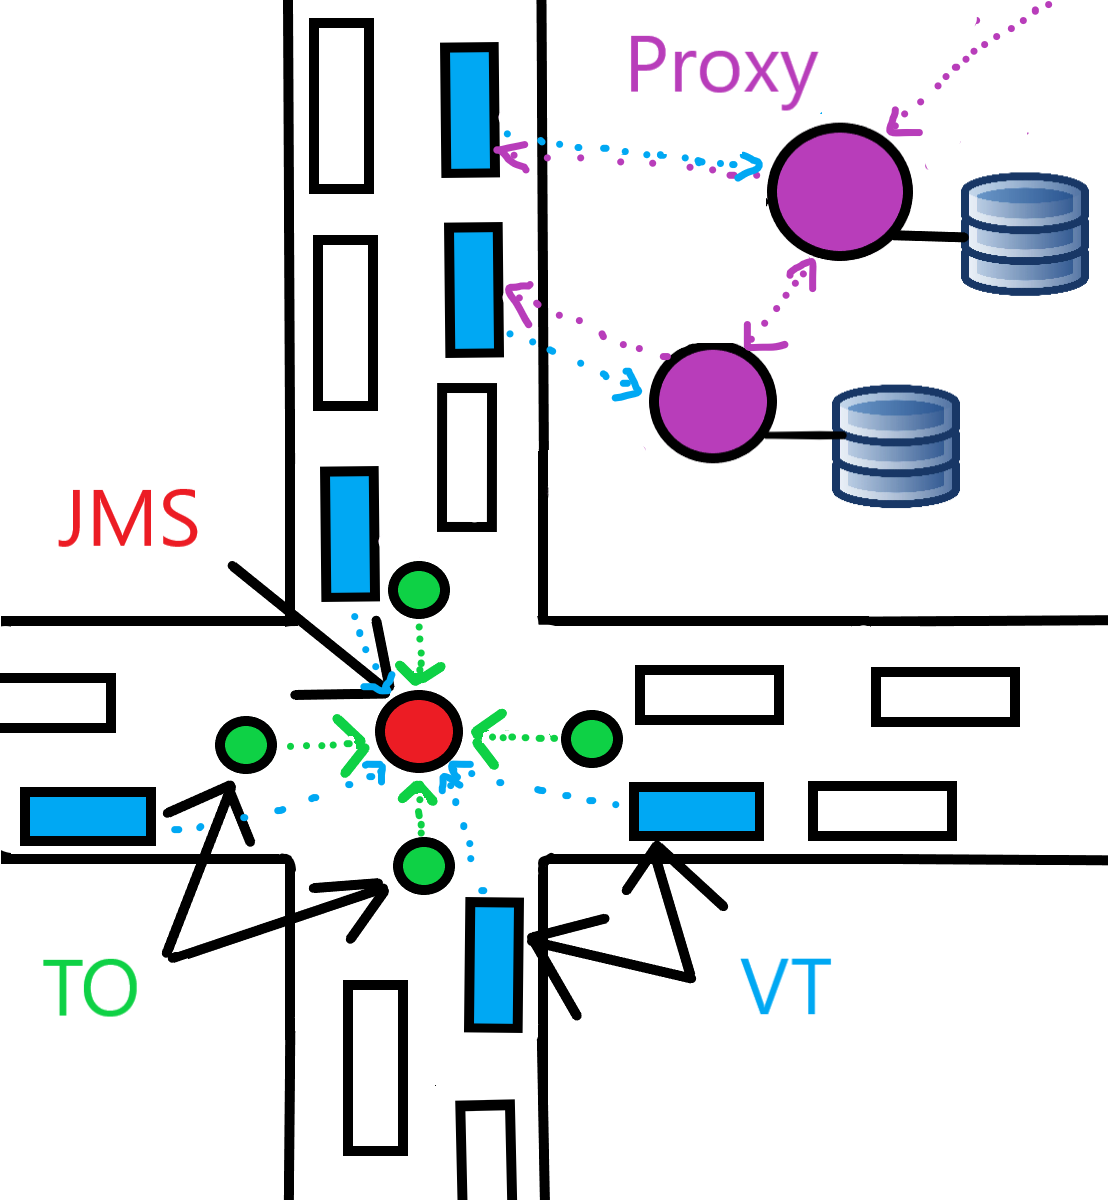
\includegraphics[width=\textwidth]{Sketches/SchitaSistem.png}
    \caption{System sketch}
    \label{fig:System_sketch}
\end{figure}

\pagebreak

\begin{figure}[h!]
    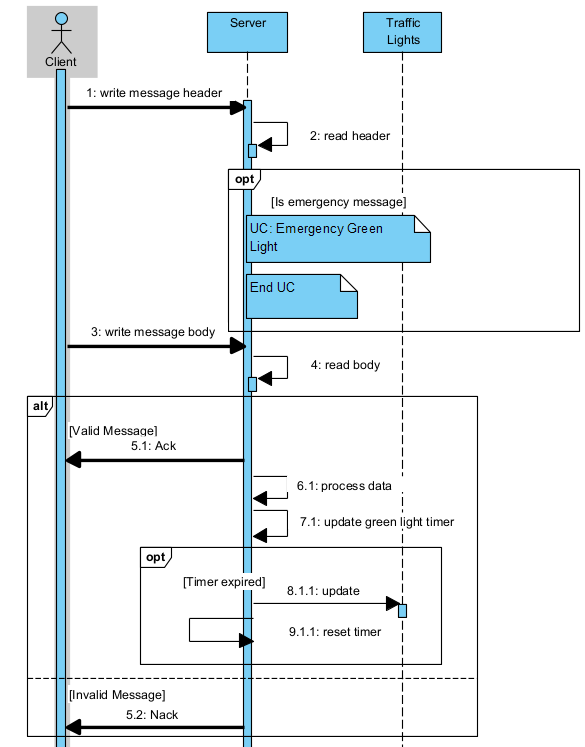
\includegraphics[width=\textwidth]{UC/SendVehicleData.png}
    \caption{UC: Send vehicle data}
    \label{fig:UC_SendVehicleData}
\end{figure}

The mechanism works mostly like any other TCP-IP mechanisms.
We read the header of the message to determine the type of 
message recieved and the size of the actual message then
based on the info we procces the data and update the traffic 
state. You may ask what happens if a car is detected by the 
TO as well as it's data is sent to the JMS trough a VT.
Well, because of this scenario we chose to aproximate the 
traffic based on the number of cars determined by the TO 
and the number of VT that sent messages to the JMS. Like this
we make sure that, if one of the 2 components fail the system
will still work. Also because noone is suppose to wait to long
for the green light we can set a maximum timer for the red light.
Imagine beeing alone on one road waiting for the green light and
having thousands of cars crossing the intersection from another road,
you would have to wait ages for you to be able to cross. This prevents that
and acts just like an "aging mechanism" (Figure ~\ref{fig:UC_SendVehicleData}).

\begin{figure}[h!]
    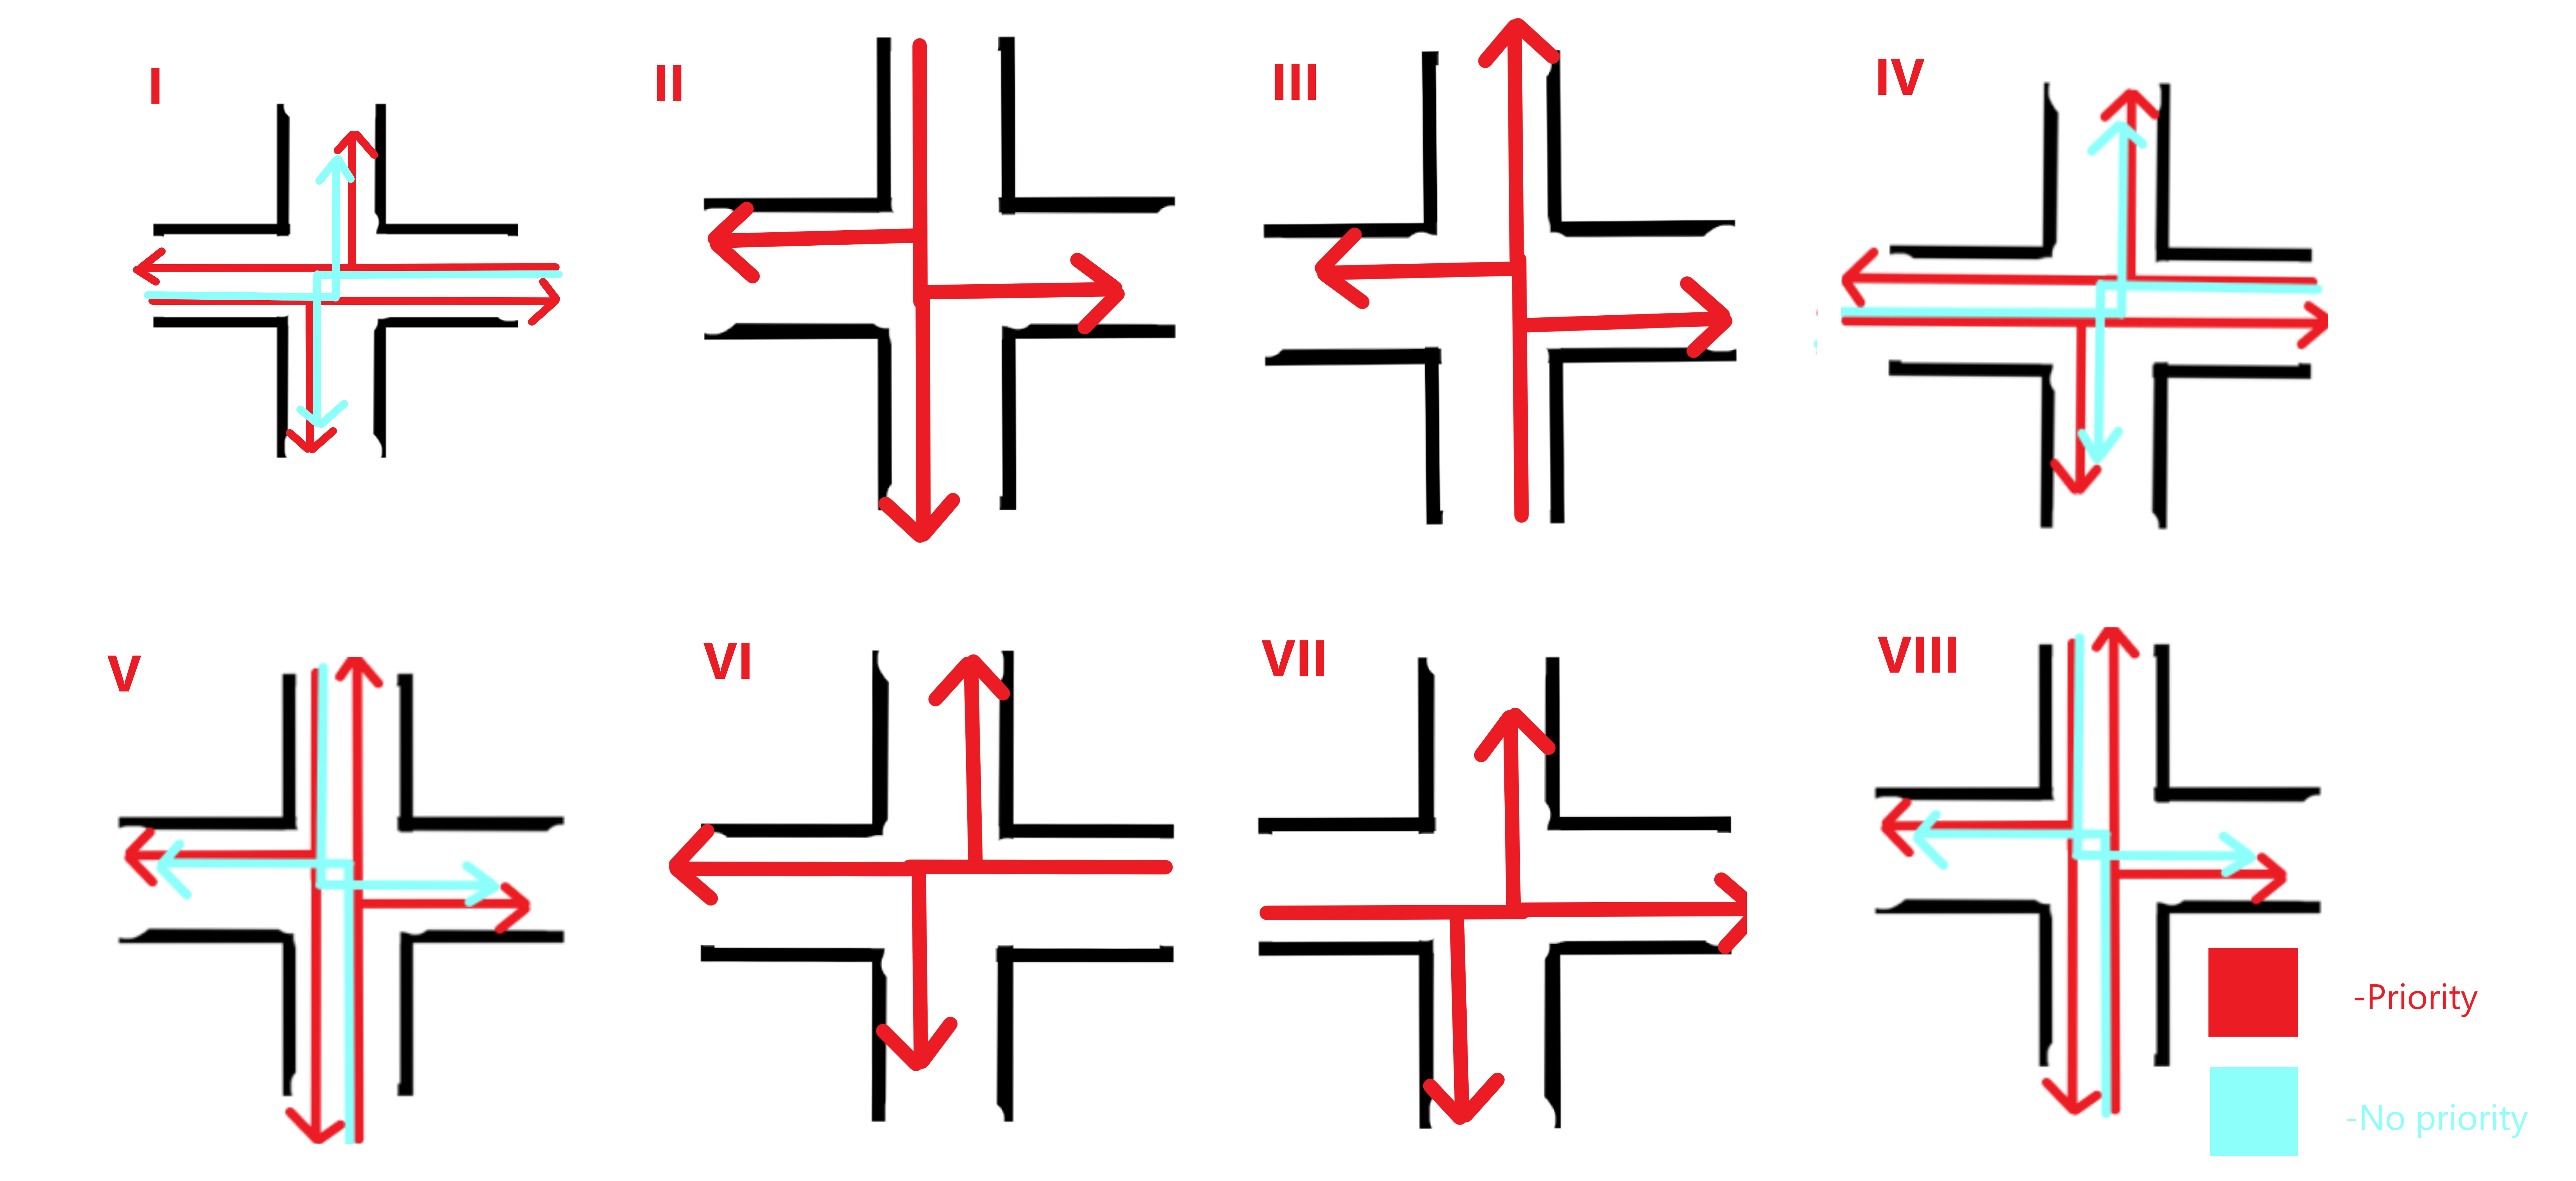
\includegraphics[width=\textwidth]{Sketches/AvailableJunctionPhazes.png}
    \caption{Junction Phazes}
    \label{fig:Junction_Phazes}
\end{figure}

As far as the main algorithm for the traffic management goes we have 8 phazes of
the traffic (Figure ~\ref{fig:Junction_Phazes}). The most basic scenarios is that the 
traffic will follow that 8 phaezes going trough phaezes 1 to phaze 8 in order. That's
what is already implement for the current way the traffic works, we want to also be
able to jump from one phaze to any other at any given time, to be able to shorcut
the system. For that we are basing on several things.\\

\indent \indent
First and foremost we need to take into 
account the number of cars waiting. We do that by combing the results from the 
VT and TO and take their maximum. Because in the TO scope we use Image Recognition 
and it may sometimes fail we will be using both entering and leaving counts and use 
ML(Machine Learning) to determine the actual number of cars that crossed the road.
The algorithm will want to make the entering vehicles at least as high as the leaving ones,
so we will be using the following equation:
\begin{math}
    vehicles = max(x, f(y)) 
\end{math}
;x being the number of the vechiles from the VT, y the number of vehicles from the TO,
and f beeing the function constantly beeing changed by our ML.\\

\pagebreak

\indent \indent
Second of all we will need to fully understand our traffic pahzes, why the are required
and how to determine the phaze we want to switch to. For that we first described the 
phazes based on the acting vehicles.\\
\begin{itemize}
    \item PHAZE I: E + W waiting vehicles
    \item PHAZE II: N waiting vehicles
    \item PHAZE III: S waiting vehicles
    \item PHAZE IV: E + W waiting vehicles (same with PHAZE I)
    \item PHAZE V: N + S waiting vehicles
    \item PHAZE VI: E waiting vehicles=
    \item PHAZE VII: W waiting vehicles
    \item PHAZE VIII: N + S waiting vehicles (sane with PHAZE V)
\end{itemize}

\indent \indent
Now we want to know when to switch from one phaze to another. For that we will have
timers for each direction: E, W, N and S. At first all the timers will be set to 
300 sec (5 min) waiting time, but the waiting time will be changed by the use of
another ML updated function. This will be further described as right now, the reasons
behind it will not be fully understood.\\
\indent \indent
Now, to start the whole mechanism we would want to just start the traffic as usual, 
having the normal order of phazez running and for us to switch to and abnormal 
phaze we'll just need one or more timers to expire. As any other timer, it will decrease normally,
but also when a car starts waiting at the crossroad timer will be decreased by f(x), x beeing 
the time left for the timer to expire. We want to have as little cars waiting at the junction
and as many cars crossing. For that we use yet another ML algorithm to update the function that 
determines how much time will be taken from the timer. The criteria for it will be that 
we want to stick to a not that low but not that high fix number of cars. For now we will be wanting
to have at least 10 cars crossing at once. The check for the jump to an abnormal phaze
will be done ONLY when GREEN LIGHT ENDS.\\
\indent \indent
The green light can be intrerupted only be emergency states(will talk about this later)
and is based on yet another ML algorithm. To maintain traffic safety conditions,
we have a fix time set for the drivers to notice the green light switch, to be prices
5 sec. You may think that this is very low, but it can actually be extended to 15 sec as 
the maximum number of phazes we can go trough without any cars waiting is 3 and we want to
keep wasted time as low as possible, that's the main reason of creating the system so any
bigger time perios would be a waste. The green light time will take the following form:
\begin{math}
    time = 5 + f(x)
\end{math}
where x is the number of cars waiting and f is the function updated by the ML algorithm.
The criteria of the algorithm is to make as close to x cars pass the junction during the 
green light and is really usefull when it comes to the speed the vechiles are moving on 
different roads.

\pagebreak

\begin{lstlisting}[language = C++]

\end{lstlisting}
\pagebreak

\indent \indent
Last but not least we need to define the way our algorithm jumps from one phaze to 
another, for that we will use the following example
(Figure ~\ref{fig:PhazesSwitchingExample}):
\begin{figure}[h!]
    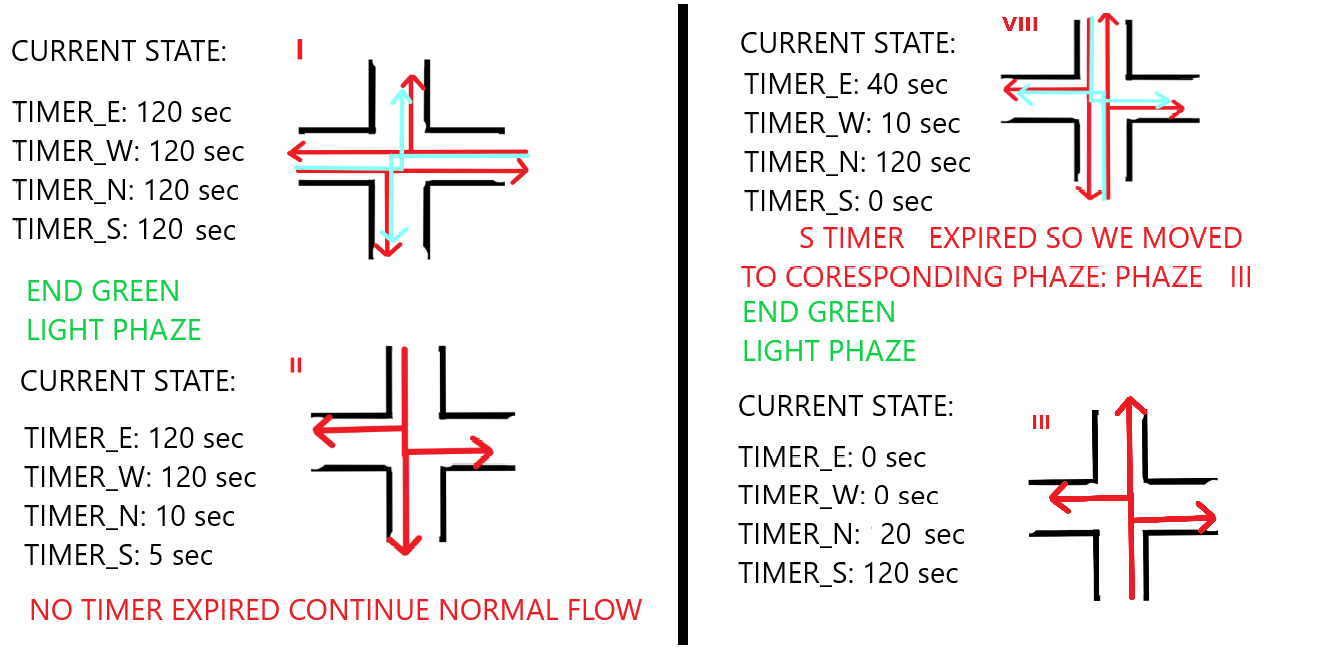
\includegraphics[width=\textwidth]{Sketches/SwitchingTroughPhazesExample.png}
    \caption{Phaze switching example}
    \label{fig:PhazesSwitchingExample}
\end{figure}
\\
\indent \indent
At the end of every green light phaze we check the timers. If any of 
them expired we jump to it's corresponding phaze. If, for example the following state
coresponds to the phaze we want to jump to, we do not short circuit the normal flow of
things. Every time we are trough green light phazes it's timer is frozen and then 
reset to it's maximum value.\\
\indent \indent
We need to talk also about the situations we want to avoid
as much as possible. This are caused as a result of letting the cars from only one
road cross (phazes II, III, VI and VII)(Figure ~\ref{fig:FaultyPhazeSwitching}). 
As mentioned before we use FIFO logic and take the phaze that corresponds to the first 
timer(s) that expired as a fix.
\begin{figure}[h!]
    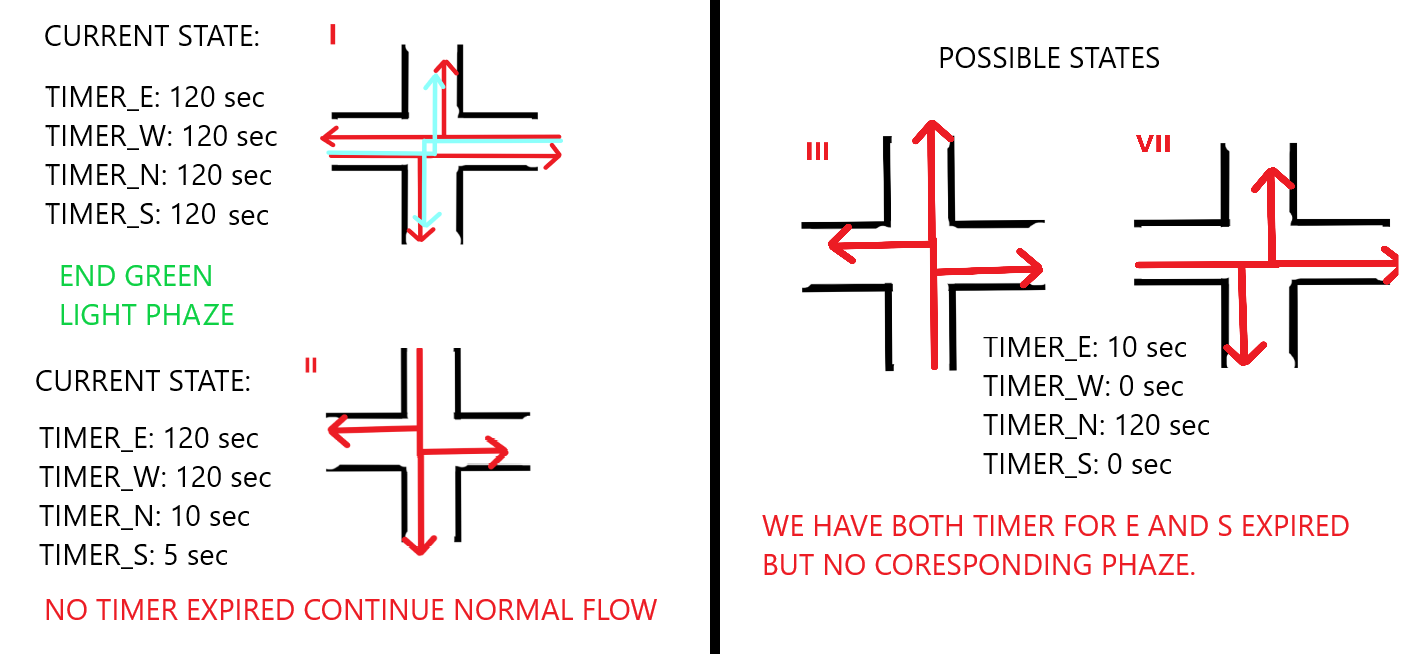
\includegraphics[width=\textwidth]{Sketches/PhazeSwitchingCaseToBeAvoided.png}
    \caption{Faulty phaze switching}
    \label{fig:FaultyPhazeSwitching}
\end{figure}

\pagebreak
\subsubsection{Emergency states}
\indent \indent
Because every lifes matter we wanted to make sure that the
special vechiles like ambulances, police cars and fire trucks
crossing the junctions will be treated differently. For that,
whenever one of those vehicle is detected our server turns on
the green light corresponding to the lane they are following
and keeps it on until it crosses the junction. If we are already
in an so called emergency green light state, the procces will
just be queued and be restarted when the already incoming 
emergency vehicle passes. (Figure ~\ref{fig:UC_EmergencyGreenLightStart}).
\begin{figure}[h!]
    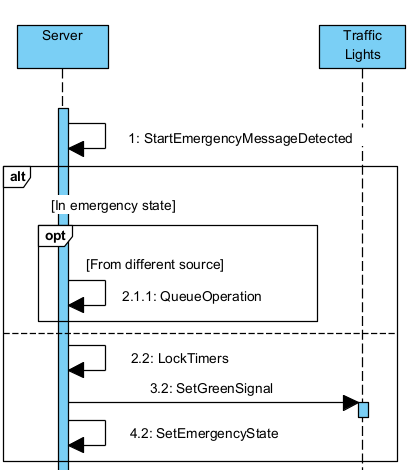
\includegraphics[width=\textwidth]{UC/EmergencyStart.png}
    \caption{UC: Emergency Green Light Start}
    \label{fig:UC_EmergencyGreenLightStart}
\end{figure}

\pagebreak

\indent \indent 
Of course when finishing with an emergency state we should
try to first of determine if another one should be started right
after or we should come back to the normal flow of traffic. Also
we should restart the maxium wait time timers, as they were frozen 
during the whole emergency state. (Figure ~\ref{fig:UC_EmergencyGreenLightStop}).
\begin{figure}[h!]
    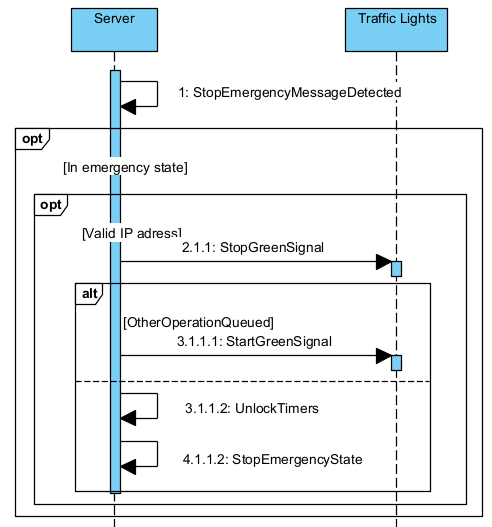
\includegraphics[width=\textwidth]{UC/EmergencyStop.png}
    \caption{UC: Emergency Green Light Stop}
    \label{fig:UC_EmergencyGreenLightStop}
\end{figure}
% TO HAVE EXAMPLE FOR EMERGENCY STATE AS WELL WE JUST WANT 
% TO LOCK THE GREEN LIGHT TIMER, OTHER TIMERS ARE WORKING AS
% WITH THE NORMAL ABOVE SCENARIO
\pagebreak

\pagebreak



\section{Implementation details}
\indent \indent
The whole system was developed using C++17, Python, Boost, GLFW, MSVC WinAPI, OpenCV,
Tensorflow  and MySQL. The system itself is treated as a big project 
and splitted into multiple submodules: 

\begin{itemize}
    \item static librarys
    \begin{itemize}
        \item Common
        \item CarDetector
        \item IPC
    \end{itemize}
    
    \item executables
    \begin{itemize}
        \item servers
        \begin{itemize}
            \item Proxy
            \item JunctionMainServer
            \item ObjectDetectionServer
        \end{itemize}
        \item  clients
        \begin{itemize}
            \item VehicleTracker
            \item TrafficObserver
        \end{itemize}
        \item testing
    \end{itemize}
\end{itemize}

This section aims to explain in detail what each and every one of this submodules were meant to do,
how they were implemented some examples of using them and the main features that they
provide. The project is not cross platform, it's Windows oriented at the moment because
during the development of the whole system Microsoft Visual Studio 2022 MSVC was used
as it provided a really quick and easy way of debugging my applications, but 
the code itself can be later converted to be cross platform using CMake, appart from
the testing module, as it is using WinAPI to spawn and handle processes. 


\pagebreak
\subsection{Common}
\indent \indent
The main ideea of the common submodule is to act as a helper library. It provides 
solutions to the following commonly found problems:
\begin{description}
    \item[Multi threaded concurency:] Thread safe structures:\\
    - ThreadSafePriorityQueue\\
    - ThreadSafeQueue
    \item[Handling GPS output:] NMEA coordinates data parsing: \\
    - GPGLL, lat, N/S, lon, E/W, time, A/V, A/D/E/M/N * checksum\\
    - GPGGA, time, , N/S, lon, E/W, Position Fix Indicator, Satellites used, HDOP, MSL Altitude, Units, 
	Geoid Separation, Units, Age of diff. corr., Diff. ref. station ID * checksum\\
    - GPRMC, time, A/V, lat, N/S, lon, E/W, Speed over ground,
    Course over ground, Date, Magnetic Variation, A/D/E * checksum
    \item[MySQL interactions:] C++ class tabel encapsulation and query handling
    \begin{figure}[h!]
        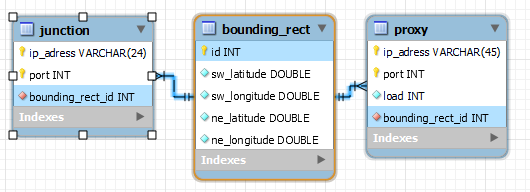
\includegraphics[width=\textwidth]{DB/DbSchema.png}
        \caption{Database Schema}
        \label{fig:Database Schema}
    \end{figure}
    \item[Parsing config files:] Specific json parser, data type converter
    \item[Creating preplanned timed actions:] Observers, Timers 
    \item[Handling user input] command line parser, signals handler
    \item[Syncronosly logging on multiple threads:] Costumizable logger
\end{description}


\pagebreak
\subsection{IPC}
\indent \indent
To establish the communication amoung all the executables I choose to come up with 
my own IPC implementation, while using Boost Asio for socket handling. The loggic 
itself runs on 4 threads: one for keeping the context running, one for reading,
one for writing and one for notifying progress.


\begin{lstlisting}[language = C++][H]
    template<typename T>
    class Client
    {
    private:
        common::ThreadSafePriorityQueue<OwnedMessage<T>> incomingMessages_;

    protected:
        boost::asio::io_context context_;
        std::thread threadContext_;
        std::mutex mutexUpdate_;
        std::condition_variable condVarUpdate_;
        std::unique_ptr<Connection<T>> connection_;
        std::atomic<bool> shuttingDown_ = false;
        boost::asio::io_context::work idleWork_;
        LOGGER("CLIENT");
    public:
        bool connect(const utile::IP_ADRESS& host, const ipc::utile::PORT port);
        void disconnect();
        bool isConnected();
        void send(const Message<T>& msg);
        bool waitForAnswear(uint32_t timeout = 0);
        std::optional<std::pair<OwnedMessage<T>, bool>> getLastUnreadAnswear();
    }
\end{lstlisting}

\pagebreak

\begin{lstlisting}[language = C++][H]
    template <typename T>
    class Connection : public std::enable_shared_from_this<Connection<T>>
    {
    protected:
        const Owner owner_;
        std::thread threadRead_;
        std::thread threadWrite_;
        std::mutex mutexRead_;
        std::mutex mutexWrite_;
        std::condition_variable condVarRead_;
        std::condition_variable condVarWrite_;
        std::condition_variable& condVarUpdate_;
        boost::asio::io_context& context_;
        boost::asio::ip::tcp::socket socket_;
        common::ThreadSafePriorityQueue<OwnedMessage<T>>& incomingMessages_;
        common::ThreadSafePriorityQueue<Message<T>> outgoingMessages_;
        Message<T> incomingTemporaryMessage_;
        std::atomic_bool isReading_;
        std::atomic_bool isWriting_;
        std::atomic_bool shuttingDown_ = false;
        uint32_t id_;
        std::string ipAdress_;
        LOGGER("CONNECTION-UNDEFINED");

    private:
        bool readData(std::vector<uint8_t>& vBuffer, size_t toRead);
        void readMessages();
        void writeMessages();
    public:
        Owner getOwner() const;
        bool connectToServer(
            const boost::asio::ip::tcp::resolver::results_type& endpoints);
        bool connectToClient(uint32_t id);
        void disconnect();
        bool isConnected() const;
        void send(const Message<T>& msg);
    }
\end{lstlisting}

\pagebreak

\begin{lstlisting}[language = C++][H]
    template<typename T>
    class Server
    {
    protected:
        common::ThreadSafePriorityQueue<OwnedMessage<T>> incomingMessagesQueue_;
        boost::asio::io_context context_;
        std::thread threadContext_;
        std::thread threadUpdate_;
        std::condition_variable condVarUpdate_;
        std::mutex mutexUpdate_;
        std::mutex mutexMessage_;
        boost::asio::ip::tcp::acceptor connectionAccepter_;
        common::ThreadSafeQueue<uint32_t> availableIds_;
        std::map<uint32_t, std::shared_ptr<Connection<T>>> connections_;
        std::atomic<bool> shuttingDown_ = false;
        LOGGER("SERVER");
    private:
        void update();
    public:
        bool start();
        void stop();
        void waitForClientConnection(); //ASYNC
        void messageClient(std::shared_ptr<Connection<T>> client,
            const Message<T>& msg);
    protected:
        virtual bool onClientConnect(std::shared_ptr<Connection<T>> client);
        virtual void onClientDisconnect(std::shared_ptr<Connection<T>> client);
        virtual void onMessage(std::shared_ptr<Connection<T>> client,
            Message<T>& msg);
    }
\end{lstlisting}

\pagebreak

\begin{lstlisting}[language = C++][H]
    template <typename T>
    struct MessageHeader
    {
        T type{};
        uint16_t id{};
        bool hasPriority = false;
        size_t size = 0;
    };
    
    template <typename T>
    struct Message
    {
        MessageHeader<T> header{};
        std::vector<uint8_t> body;

        size_t size() const;
        void clear();
        Message<T> clone();

        friend std::ostream& operator << (std::ostream& os, 
            const Message<T>& msg);
        template<typename DataType>
        friend Message<T>& operator << (Message<T>& msg, const DataType& data)
        template<typename DataType>
        friend Message<T>& operator >> (Message<T>& msg, DataType& data)
    }
\end{lstlisting}   
\pagebreak

\subsection{CarDetector}
\indent \indent
To be able to connect to the road traffic cameras and count the number of 
incoming/outgoing vehicles I made wrappers over OpenCV library. The whole process 
works as follows: it starts detecting the moving objects inside a give frame, try to 
predict their next position and once they cross a imaginary lines inside the picture
they are accounted if they were matched to be cars. To boost performance, the 
module runs on 4 threads: providing images from the camera, detecting moving objects,
classifying objects as cars and displaying the bounding boxes. The last one can be 
disable, as it is just for illustrative purposes. \\

\indent \indent
The car classification itself is 
not done by the given module due to current C++ Tensorflow - OpenCV outdated compatibility,
but by the ObjectDetectionServer written in Python. The CarDetector module just acts 
like a client and sends the actual bytes of the cropped image of the detected moving objects 
to the server. I have to note that if, in the near future, the compatibility issues
will be fixed, it would server as a great performance upgrade to move this logic
inside the module and remove any kind of process interactions.


\subsection{ObjectDetectionServer} 
\indent \indent
To be able to able to detect if cars were present Tenserflow was used. Due to the fact 
that the model will be loaded by a microcontroller a
\href{https://github.com/tensorflow/models/blob/master/research/object_detection/g3doc/tf2_detection_zoo.md}{SSD MobileNet model}
was trained by using a \href{https://universe.roboflow.com/pedro-azevedo-3c9ol/bdd100k-3zgda/dataset/5}{public dataset}.
The training took about 15h on an RTX 3060 and the model is capable of detecting cars,
street lights and other traffic related objects but it will be used just for detecting cars.
The model speed is the most important thing here beeing able to evaluate 22 frames/s,
as it's accuracy is not that great averaging 60\%. The overcome the low accuracy any object 
that is more then 50\% likely to be a car will be taken into account.\\

\indent \indent6
The model itself is loaded just once, on a server, because it seems to be a really time consuming 
operation and used whenever a new message is recieved. Once the predictions are done, we 
remove the overlapping objects detected with the help of OpenCv NMSBoxes and return just the size 
of the remaining list of objects, not the bounding boxes themself. To keep the consistency of
the IPC implementation I imported the C++ message definitions and implemented the created a
simple implementation of a server using socket package.  



\pagebreak

\subsection{Proxy}
\indent \indent
The proxy is a wrapper over the server implementation that assures the connection
between the vechile trackers and the next junction main server they will encounter.
Every single one is connected to their own database, that contains a list of junctions,
proxys and the area covered by them. \\
\indent \indent
They way it works is preaty straight forward, if a client 
querys the proxy for the next junction it searches the database. If it finds 
a suiting junction then it sends the connection data, otherwise it redirects 
the vehicle to the closeste proxy. This process repeats itself until it 
finally reaches one valid junction or the car is out of coverage area (for 
example if the car is somewhere on a ship in the middle of the sea there is 
no reason for us to connect it to a junction).

\begin{figure}[h!]
    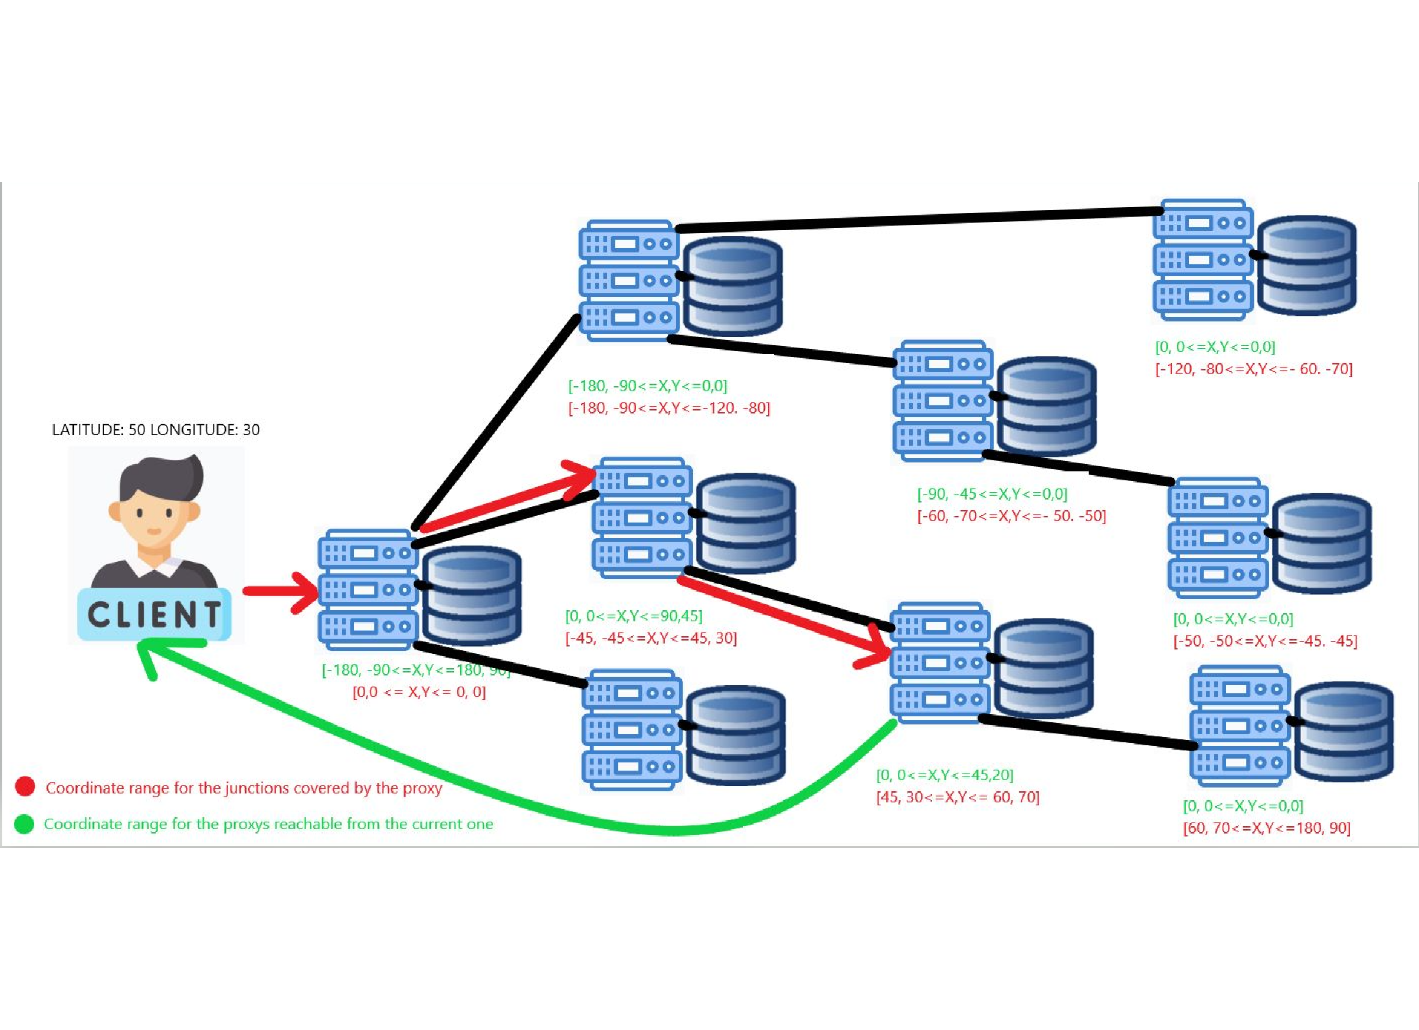
\includegraphics[width=\textwidth]{Sketches/ProxyFlowV2.png}
    \caption{Proxy querys flow}
    \label{fig:Proxy querys flow}
\end{figure}

The server themself has a range of coordinate values for the covered junctions
and a range of coordinate values for the known connected subproxys. The coordinate 
range of the know connected proxys lessens the more you go down the connection tree 
until an enpoint is reached, marked with range {0,0} <=> {0,0}. If we still don't got 
an answear from the proxy containing a junction that means that we are out of reach 
and the client will just stop. Like this, the more server we will have to spread our 
junction data, the faster the communication will be, as the client doesn't necessarily
need to interogate the main server, it can interogate any of the servers.
\pagebreak


\subsection{JunctionMainServer}

\indent \indent
The executable is a wrapper over the server implementation that manages the traffic states.
It keeps track of the incoming vehicles and times out each and every traffic state. The 
implementation itself is though to be a state machine, with the states represented by the 
traffic states and the events beeing timer expire events. Each state has associated to it 
a timer that decreases normally or when an incoming vehicle is detected. Whenever we 
are in a given state, it's corresponding timer is frozen and afterwards deleted. We aim to 
minime the amount of conflicting states previously described so the amount of time decreased
when a car arrives is ddynamically calculated. 

\begin{lstlisting}[language = C++][H]
{ 
    "server": { "ip": "127.0.0.1", "port": 5000 },
    "maxWaitingTime": 2,
    "usingRightLane": true,
    "lanes": { 
        "top": "keyword1", "down": "keyword2",
        "left": "keyword3", "right": "keyword3"
    } 
}
\end{lstlisting}

During the testing of the given module it was observed that traffic tends to keep it's 
normal flow, there is no jumping between traffic states unless a large inflow of cars is 
detected. Even if this happens, after the required jump transitions, traffic states will 
be normalized back to their initial definition.

% TO DO ADD PICTURE HERE
\pagebreak
\subsection{TrafficObserver}
\indent \indent
The executable is a wrapper over the client implementation that combines
cardetection functionalities. On startup it recieves a keyword for the junction to be able
to determine what lane provided the incoming car message. To be able to run 
the executable itself you will need to provide a camera as well as a way to 
connect to the network, for example a zigbee. For testing porposes a
video was provided instead of linking directly to a camera.

\begin{figure}[h!]
    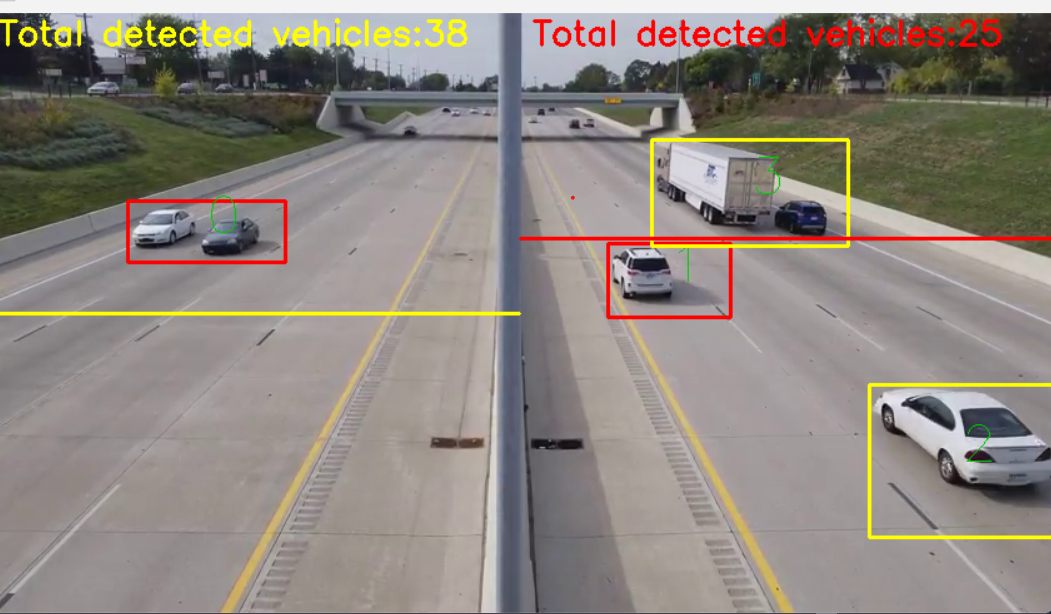
\includegraphics[width=\textwidth]{TrafficDetectionRunningExample.png}
    \label{fig:Running client sample}
\end{figure}

\begin{figure}[h!]
    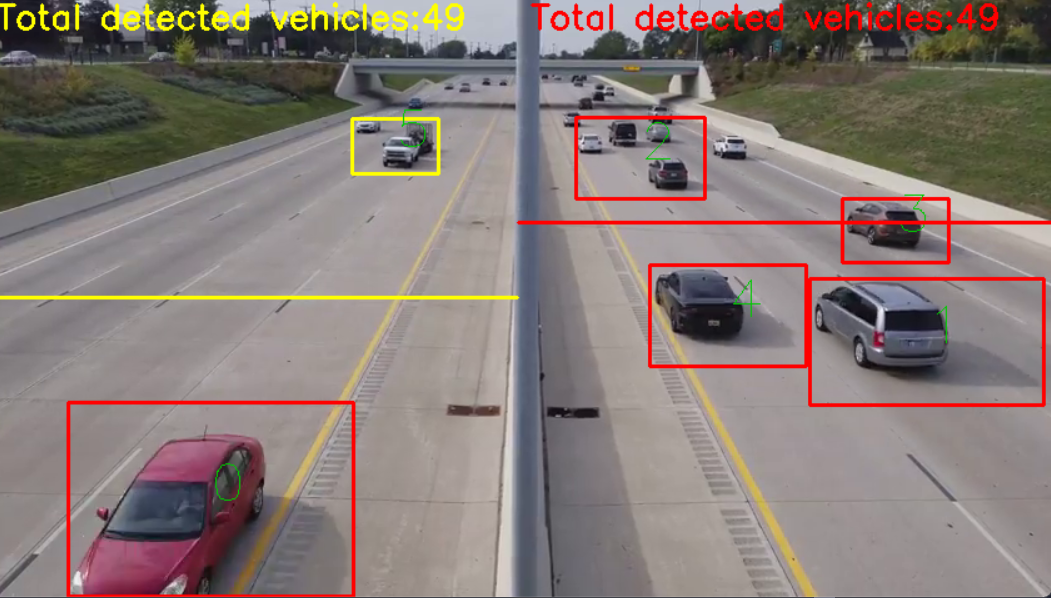
\includegraphics[width=\textwidth]{TrafficDetectionRunningExample2.png}

    \label{fig:Running client sample2}
\end{figure}

\pagebreak
\subsection{VehicleTracker}
\indent \indent
The executable is a wrapper over the client. On startup it tries loading a
config file that contains an ordered list with the previous queried proxies.
If not present, it will just interogate the main server. Once the application
shuts down a config file will be saved with all the queried proxys, so it's
suppose to almost always load a config file.

\begin{lstlisting}[language = C++][H]
{
    "proxys": [
    { "ip_adress": "127.0.0.1","port": 6000},
    { "ip_adress": "127.0.0.5","port": 5000}]
}
\end{lstlisting}

The executable aims to be downloaded on each car system by the manufacturer
and it requires a GPS module to be pressent as well as a wifi module. Messages
start to be sent only when the vehicle itself is moving. To be able to
determine this as well as it's heading GPS data is manually parsed, extracting
latitude and longitude from NMEA GPGLL, GPGGA and GPRM inputs. For testing
purposes data was already written inside a file and passed trough a pipe to the
application. The data itself was taken from a \href{https://github.com/ChrisvdHoorn/NMEA_message_GPS_data}{public repository}.

\indent \indent
We first query the last visited proxy. If we are out of reach, we move up the proxy list
until eventually we get valid junction connection data or we get back to
the root of the connection tree(the main server). If we have reached the root node, 
the process of searching for a junction without a config file restarts. Once we got the 
connection data we notify the junctions whenever we aproach/disconnect from it. Once we 
have passed a junction the whole process restarts from the begining.

\begin{figure}[h!]
    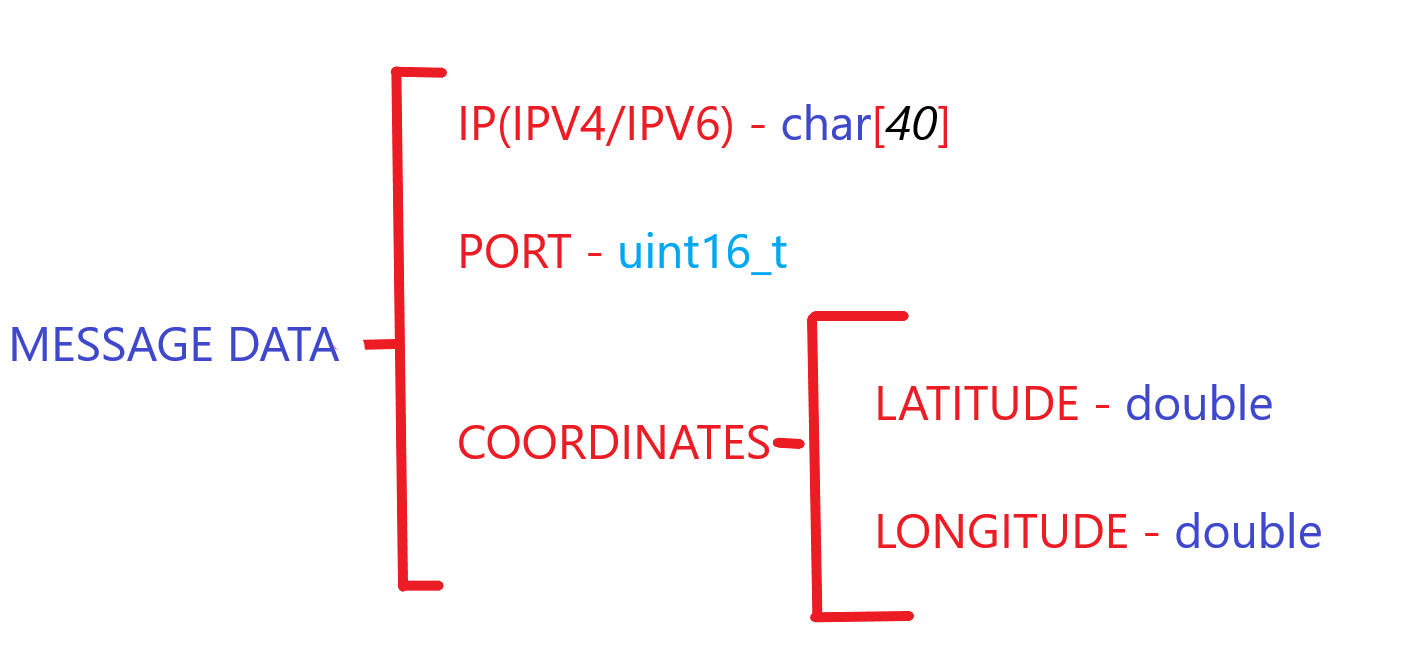
\includegraphics[width=\textwidth]{Sketches/ProxyJunctionMessage.png}
    \caption{Proxy junction data reply}
    \label{fig:Proxy junction data reply}
\end{figure}

% ex citare \cite{Deshmukh2016}

\pagebreak
\printbibliography

\end{document}